\section{Implementation}
\label{sec:impl}
%%%%%%%%%%%%%%%%%%%%%%%%%%%%%%%%%%%%%%%%%%%%%%%%%
%%%%%%%%%%%%%%%%%%%%            ALGORITHM DETAILS
%In the formalism section, we viewed the problem from the perspective of an arbitary guarantee in the model that can potentially be violated. This resulted in explicit faults at the leaf level and violated guarantees (``nondeterministic faults") at the middle/top layers. Each MCS generated at each level gives insight into the system at that level. In this section, we describe the implementation of compositional generation of minimal cut sets. %Minimal cut sets traditionally contain explicitly defined faults as elements; to this end, we implemented a compositional mapping from explicit faults to the guarantees they violate. The end result are the minimal cut sets that contribute to a violation of the top level safety property. 
In the formalism, any guarantee in the model had an associated fault activation literal and could be unconstrained. In the implementation, we rely on the fault model created in the safety annex to dictate which guarantees can be violated and how they may fail. Each explicit fault defined in the safety annex is added to the Lustre program as are assocated fault activation literals~\cite{Stewart17:IMBSA,stewart2020safety}. This corresponds to the $f_i$ and $\mathit{af}_i$ described in Section~\ref{sec:formalization}. 

\begin{figure}[h!]
	%\vspace{-2em}
	\begin{center}
		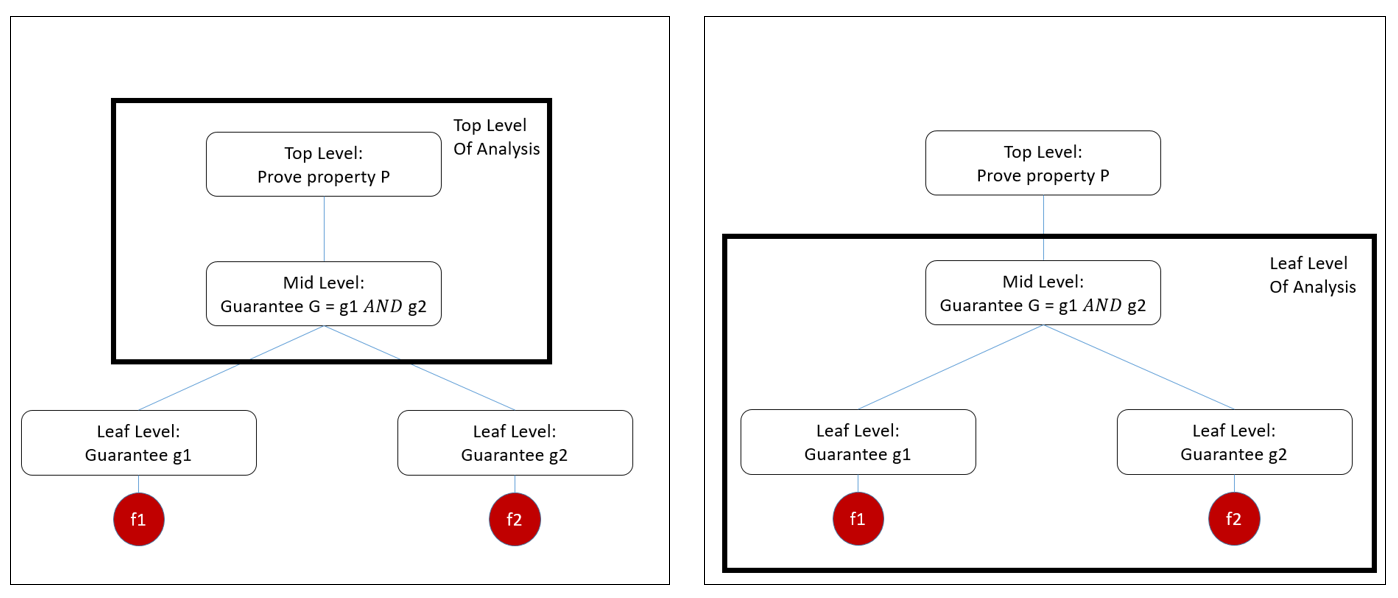
\includegraphics[width=0.9\textwidth]{images/twoLevels.PNG}
	\end{center}
	\vspace{-2em}
	\caption{Illustration of Two Layers of Analysis}
	\label{fig:layers}
\end{figure}

The \aivcalg algorithm requires that equations in the Lustre model are flagged for consideration in the analysis; these we call \emph{IVC algorithm elements}. All equations in the model can be used as IVC algorithm elements or one can specify directly the equations to consider. In this implementation, the IVC algorithm elements are added differently depending on the layer. In the leaf architectural level, fault activation literals are added to the IVC algorithm elements and are constrained to {\em false}. In middle or top layers, supporting guarantees are added. This is shown in Figure~\ref{fig:layers}. The figure shows an arbitrary architecture with two analysis layers: top and leaf. The top layer analysis adds $G$ as IVC algorithm element; the leaf layer analysis adds $f_1$ and $f_2$. 

A requirement of the hitting set algorithm is that to find all MCSs, all MUSs must be known. Ghassabani et al.~\cite{Ghassabani2017EfficientGO} showed that finding all MIVCs is as hard as model checking. It is a requirement of this analysis that all MIVCs are found. Once the MIVC analysis is complete for a property at a given layer, a hitting set algorithm is used to generate the related MCSs~\cite{murakami2013efficient}. Depending on the layer of analysis, the MCSs contain either guarantees or fault activation literals.

%For a safety property $P$, the set of all MCSs are understood as $\lor^{n}_{i=1} \mathit{MCS_i}(P)$; intuitively, this means if all constraints found in any single MCS are removed from the constraint system, $\neg P$ is satisfied. For each element $gf_j \in \mathit{MCS_i}$, this is understood as $\land^{m}_{i=1} \mathit{gf_i}$ and speaks to the minimality of the correction set. Thus the MCSs form a disjunctive normal formula over the safety property at that layer. As the proof proceeds down the hierarchy, each of the subcomponent guarantees become a property to be proven and thus MIVCs/MCSs are generated. The composition of the MCSs consists of replacing a contract in a higher layer MCS with the disjunctive normal formula of its own MCSs. After all replacements have been made, the system property formula is converted back into disjunctive normal form. 

The composition of these results is performed top down and shown in Algorithm~\ref{alg:compose}. For each guarantee found in an MCS, a replacement is made with the guarantees own MCSs. This is done recursively until all replacements have been made (line 7, 8 of Algorithm~\ref{alg:compose}). If on the other hand there are no MCSs for a given guarantee, that guarantee is replaced by its associated fault activation literal (line 10). At the leaf level of analysis, no guarantees have associated MCSs and thus reaches the end of recursion. At that time, the formula is converted back into disjunctive normal form to finish the translation into the traditional fault tree (line 11). 

\begin{algorithm}[h]
\SetKwFunction{Resolve}{resolve}
 \SetKwProg{Fn}{Function}{:}{}

	$R \gets \mathit{\amcs(P)} = \lor_{i=1}^n \mathit{MCS_i}$\\
	where $\mathit{MCS_i} = \land_{j=1}^m \mathit{gf_j}$\\
	\Fn{\Resolve{$R$}}{
		
		\For{$\forall$ OR-node in $R$}{
			\For{$\forall \mathit{gf_j}$ in OR-node}{
				\eIf{ $\exists \mathit{MCS(gf_j)}$ }{
				$R \gets$ replace $gf_j$ in $R$ with $\mathit{\amcs(gf_j)}$\;
				\Resolve($\mathit{\amcs(gf_j)}$)\;
			}{
				$R \gets $ replace $\mathit{gf_j}$ in $R$ with $\mathit{af_j}$\;	
			} 
			}
		}
		convert $R$ to DNF 
	}
	\caption{Compose Results}
	\label{alg:compose}
\end{algorithm}

Algorithm~\ref{alg:compose} provides the outline for the general case of composing fault forests: for each each property in a layer, the algorithm is called. Each property may have a corresponding fault tree. The collection of fault trees associated with each property make the forest. In the next subsection, we describe how this general algorithm is adjusted.

\begin{comment}
The number of replacements $r$ that are made for a single property $P$ are constrained by the number of minimal cut sets there are for each of the $\alpha$ contracts within the initial MCS. We call the set of all minimal cut sets for a contract $g$: $\mathit{Cut(g)}$. The following formula defines an upper bound on the number of replacements. 

\begin{lemma}
The number of replacements $r$ is bounded by the following formula:
\begin{gather}
\label{eq:bound}
  r \leq {\displaystyle \sum_{i=1}^{\alpha} }({\displaystyle \prod_{j=1}^{i} |\mathit{Cut(g_j)}|})  
\end{gather}
\begin{proof}
Assume there exists a $g_i \in \mathit{MCS(P)}$. The number of replacements made for $g_i$ is at most $|\mathit{Cut(g_i)}|$. Iteratively perform this replacement for all $\alpha$ contracts in $\mathit{MCS(P)}$. In the worst case, $|\mathit{Cut(g_1)}| \times |\mathit{Cut(g_2)}| \times \cdots \times |\mathit{Cut(g_\alpha)}|$ replacements are made.
\label{lemma:bound}
\end{proof}
\end{lemma}

\end{comment}

It is important to note that the algorithm terminates. 
\begin{theorem}
Algorithm~\ref{alg:compose} terminates
\begin{proof}
No infinite sets are generated by the \aivcalg or minimal hitting set algorithms~\cite{Ghassabani2017EfficientGO,murakami2013efficient}; therefore, every MCS produced is finite. Thus, every minimal cut set of every contract is finite.
\end{proof}
\end{theorem}

This algorithm assumes a complete enumeration of minimal IVCs and the completion of the hitting set algorithm. These steps of analysis are not trivial to perform. We discuss these difficulties further in Section~\ref{sec:disc}.

\subsection{Pruning to Address Scalability}
Given that the growth of the DNF formula can be exponential in the worst case, we implemented strategies to prune the size of the cut sets and hence the growth of these intermediate sets. The safety annex provides the capability to specify a type of verification in what is called a \textit{fault hypothesis statement}. These come in two forms: maximum number of faults or probabilistic analysis. Algorithm~\ref{alg:compose} is the general approach, but the implementation changes slightly depending on which form of analysis is being performed. This pruning improves performance and diminishes the problem of combinatorial explosion in the size of minimal cut sets for larger models. 

\textbf{Guarantees with no associated faults} If a guarantee is found in a minimal correction set and no fault has been defined in the model that can violate it, this minimal correction set (and hence the entire subtree) is pruned.

\textbf{Max \textit{n} faults analysis} The max $n$ fault hypothesis in the safety annex restricts the number of faults that can be independently active simultaneously. This statement restricts the cardinality of minimal cut sets generated to $n$. If the number of elements in an MCS exceeds the threshold of the hypothesis statement, that MCS is eliminated from consideration and its subtree is pruned.


\textbf{Probabilistic analysis pruning} A probabilistic hypothesis statement restricts the cut sets by use of a probabilistic threshold. Assuming independence between faults, any cut sets with combined probability higher than the given probabilistic threshold are removed from consideration. The allowable combinations of faults are calculated before Algorithm~\ref{alg:compose} begins; this allows for dynamic pruning of minimal correction sets. If the fault activation literals within an MCS are not a subset of any allowable combination, that MCS is pruned from the formula. 

\section{Discussion}
\label{sec:disc}
There are considerations that must be made regarding this approach. These include the enumeration of all MIVCs as well as all MHSs. We discuss these preprocessing steps and then end the discussion with some brief comments on the soundness and incompleteness of compositional reasoning. 

\subsection{Minimal IVC Generation and Tractability}
Ghassabani showed that determining if an inductive validity core is minimal is as hard as model checking~\cite{ghassabani_2018, Ghassabani2017EfficientGO}. The full inductive validity core algorithm does not guarantee a minimal IVC. A separate algorithm attempts to minimize the IVCs enumerated in the full algorithm. The minimization is as hard as model checking and therefore undecidable in many settings. The implementation of the MIVC algorithm times out after a set threshold and if all MIVCs cannot be enumerated, the output of the algorithm is empty, i.e., it is an {\em offline} algorithm. 

The minimal cut sets may be enumerated via MIVCs due to the dual relationship between minimal unsatsifiable subsets (MUSs) and minimal correction sets (MCSs). The MCSs cannot be found if the unsatisfiable subsets are not minimal~\cite{liffiton2016fast}. In the case of finding minimal cut sets, if an IVC is not minimal, the hitting sets of all IVCs will not necessarily be a cut set. A simple example illustrates this concept. Assume that $\{a,b,c\}$ is an IVC and the minimal IVC contains only $\{a,b\}$. Intuitively, $a$ and $b$ are sufficient to prove some safety property. Say there are two other minimal IVCs enumerated: $\{d\}$, and $\{e\}$.  The hitting sets produced will include the set $\{c, d, e\}$. Violation of these elements will not lead to violation of the safety property, for the elements $a$ and $b$ provide a proof of the property. 

Bendik et al.~implemented an algorithm that identifies MIVCs in an {\em online} manner (i.e., one by one) and can be terminated at any time~\cite{bendik2018online}. While this algorithm performs better than the original \aivcalg algorithm developed by Ghassabani~\cite{Ghassabani2017EfficientGO}, the requirement remains that all MIVCs must be found before generating the minimal hitting sets. A possible extension to our approach is to utilize the online MIVC enumeration algorithm simply for the performance benefits. 

\subsection{Minimal Hitting Sets and Tractability}
Finding inclusion-minimal hitting sets for a given collection of sets is a fundamental combinatorial problem. The problem of generating the collection of MHSs for a given set family is of interest in a wide variety of domains. The computational complexity of this problem is currently unknown; nevertheless, there is an extensive literature of algorithms to generate minimal hitting sets~\cite{gainer2017minimal}. The minimal hitting set problem is equivalent to the inclusion-minimal set cover problem. An algorithm for generating MHSs can be used to enumerate minimal set covers, a classic NP-hard problem~\cite{karp1972reducibility}. 

Murakami et al.~ proposed an algorithm used for dualizing large-scale hypergraphs~\cite{murakami2013efficient}. A hypergraph $\mathcal{F}$ is a set family defined on vertex set $V$ . The dual of $\mathcal{F}$ is the set of minimal subsets $H$ of $V$ such that $F \cap H \not = \empty$ for any $F \in \mathcal{F}$ . The computation of the dual is equivalent to the minimal hitting set problem. Finding a minimal hitting set is easy; one removes vertices one by one unless one gets an empty intersection with some hyperedges. However, finding exactly all minimal hitting sets is not easy; one must check exponentially many vertex subsets that can be minimal hitting sets. Murakami introduced a bottom-up search. They build up ``sub-MHSs" until they are hitting sets, making clever use of intermediate data structures to ensure that no redundant checks are performed~\cite{gainer2017minimal}. The algorithm incorporated into the safety annex is the MMCS algorithm~\cite{murakami2013efficient}. Let $k = ||S||$ be the sum of sizes of the sets in a set family $S$. Then MMCS runs in $\mathcal{O}(k)$ time per iteration\footnote{The authors do not give explicit bounds on the number of iterations required.}.

Given the intractability of MIVC enumeration and the challenge of the hitting set problem, being able to generate minimal cut sets without reliance on these algorithms would be beneficial. We discuss this option in Section~\ref{sec:preproc}.

\subsection{Soundness, Completeness, and Minimality}
For any proof system, soundness is the most important property--it is not possible to deduce false facts. A measure of the quality or usefulness of a proof system is obtained from an investigation into completeness--every formula can be derived using that proof system. Compositional reasoning is sound~\cite{CompTechReport}, but in general incomplete~\cite{namjoshi2010completeness}. This means that we know in nominal compositional analysis, we will not prove a false property (sound). But there may be cases in which we cannot prove a property which is true given the model (incomplete). Given the assumption for our algorithms that the nominal model proves and all MIVCs are enumerated, we know that a fault tree is still valid using this approach. 

What we cannot ensure is that the cut sets after composition are necessarily minimal. The example described in Chapter~\ref{chap:granularity} illustrates this point. Furthermore, dependencies between guarantees within the model may not be reflected in composition. We are guaranteed minimality per layer, but it is possible to lose this property upon composition. 

From safety analysts perspective, this is acceptable. This approach is not meant to supplant an analyst, but to automate certain aspects of the traditional approach to SA. The analyst is still required to understand the cut sets and how they pertain to the system as a whole. 

From a probabilistic computation perspective, this may result in an unsafe probabilistic approximation. Assuming independence, the computed probability of a cut set will be less than or equal to the computed probability of a minimal cut set. An extension to this work is to provide a meaningful over-approximation to the probabilistic computations that may be performed over a compositionally derived fault tree. 










